\section{Motivation}
\label{sec:intro:motivation}

In this section, we first study the need for inductive biases in
machine learning. Then we analyze where current deep learning models
can get inductive biases from, and finally we highlight some problems
that this thesis addresses about inductive biases for deep linguistic
structured prediction.

\subsection{Generalization: The Need for Inductive Bias}
\label{ssec:intro:need-of-bias}

Any system~(natural or artificial) that makes general inferences on
the basis of particular and limited data must constrain its hypotheses
in some way. With limited observations and resources~(time, memory,
energy), our human intelligence of generalizing to new environments
makes us efficiently learn when interacting with the world and other
human beings. This efficiency largely depends on many {\bf inductive
  biases} from human intelligence~\citep{Gershman2021WhatMU}, which
can potentially be helpful for machine intelligence. According to
extensive cognitive science
studies~\citep{Spelke1990PrinciplesOO,Bienenstock1996CompositionalityMP,Rehder2003ACT,harlow1949formation,
  Lake2016BuildingMT,Gershman2021WhatMU}, there are many inductive
biases for human intelligence, such as compositionality, causality,
learning to learn, and so on. We do not imply machine intelligence
should mimic the human intellgence. Instead, we argue that those key
human indutive biases help overcome limited observations and resources
may inspire us to design the machine intelligence.

On the machine intelligence side, the no-free-lunch theorem for
machine learning~\citep{baxter2000model,wolpert1995no} tells us that
inductive biases that influence hypothesis selection is necessary to
obtain generalization. \citet{mitchell1980need} argues that inductive
biases constitue the heart of generalization and indeed a key basis
for learning itself.

Let us examine a concrete example: the popular supervised learning
setting.  We design algorithms that can learn from a set of supervised
training examples to predict a certain target output for an input. The
learning algorithm is presented some training examples that
demonstrate the intended relation between the input and output
values. Then the learner is supposed to learn a target function which
captures the coorelations between the inputs and outputs. Furthermore,
we hope that the learned target function can approximate the correct
output, even for examples that have not been shown during training. We
call the ability of generalizing to unseen data as
generalization. Without any additional assumptions, this
generalization problem cannot be solved since unseen situations might
have an arbitrary output value. The kind of necessary assumptions are
subsumed in the phrase inductive bias.

%\begin{figure}[!th]
%\centering
%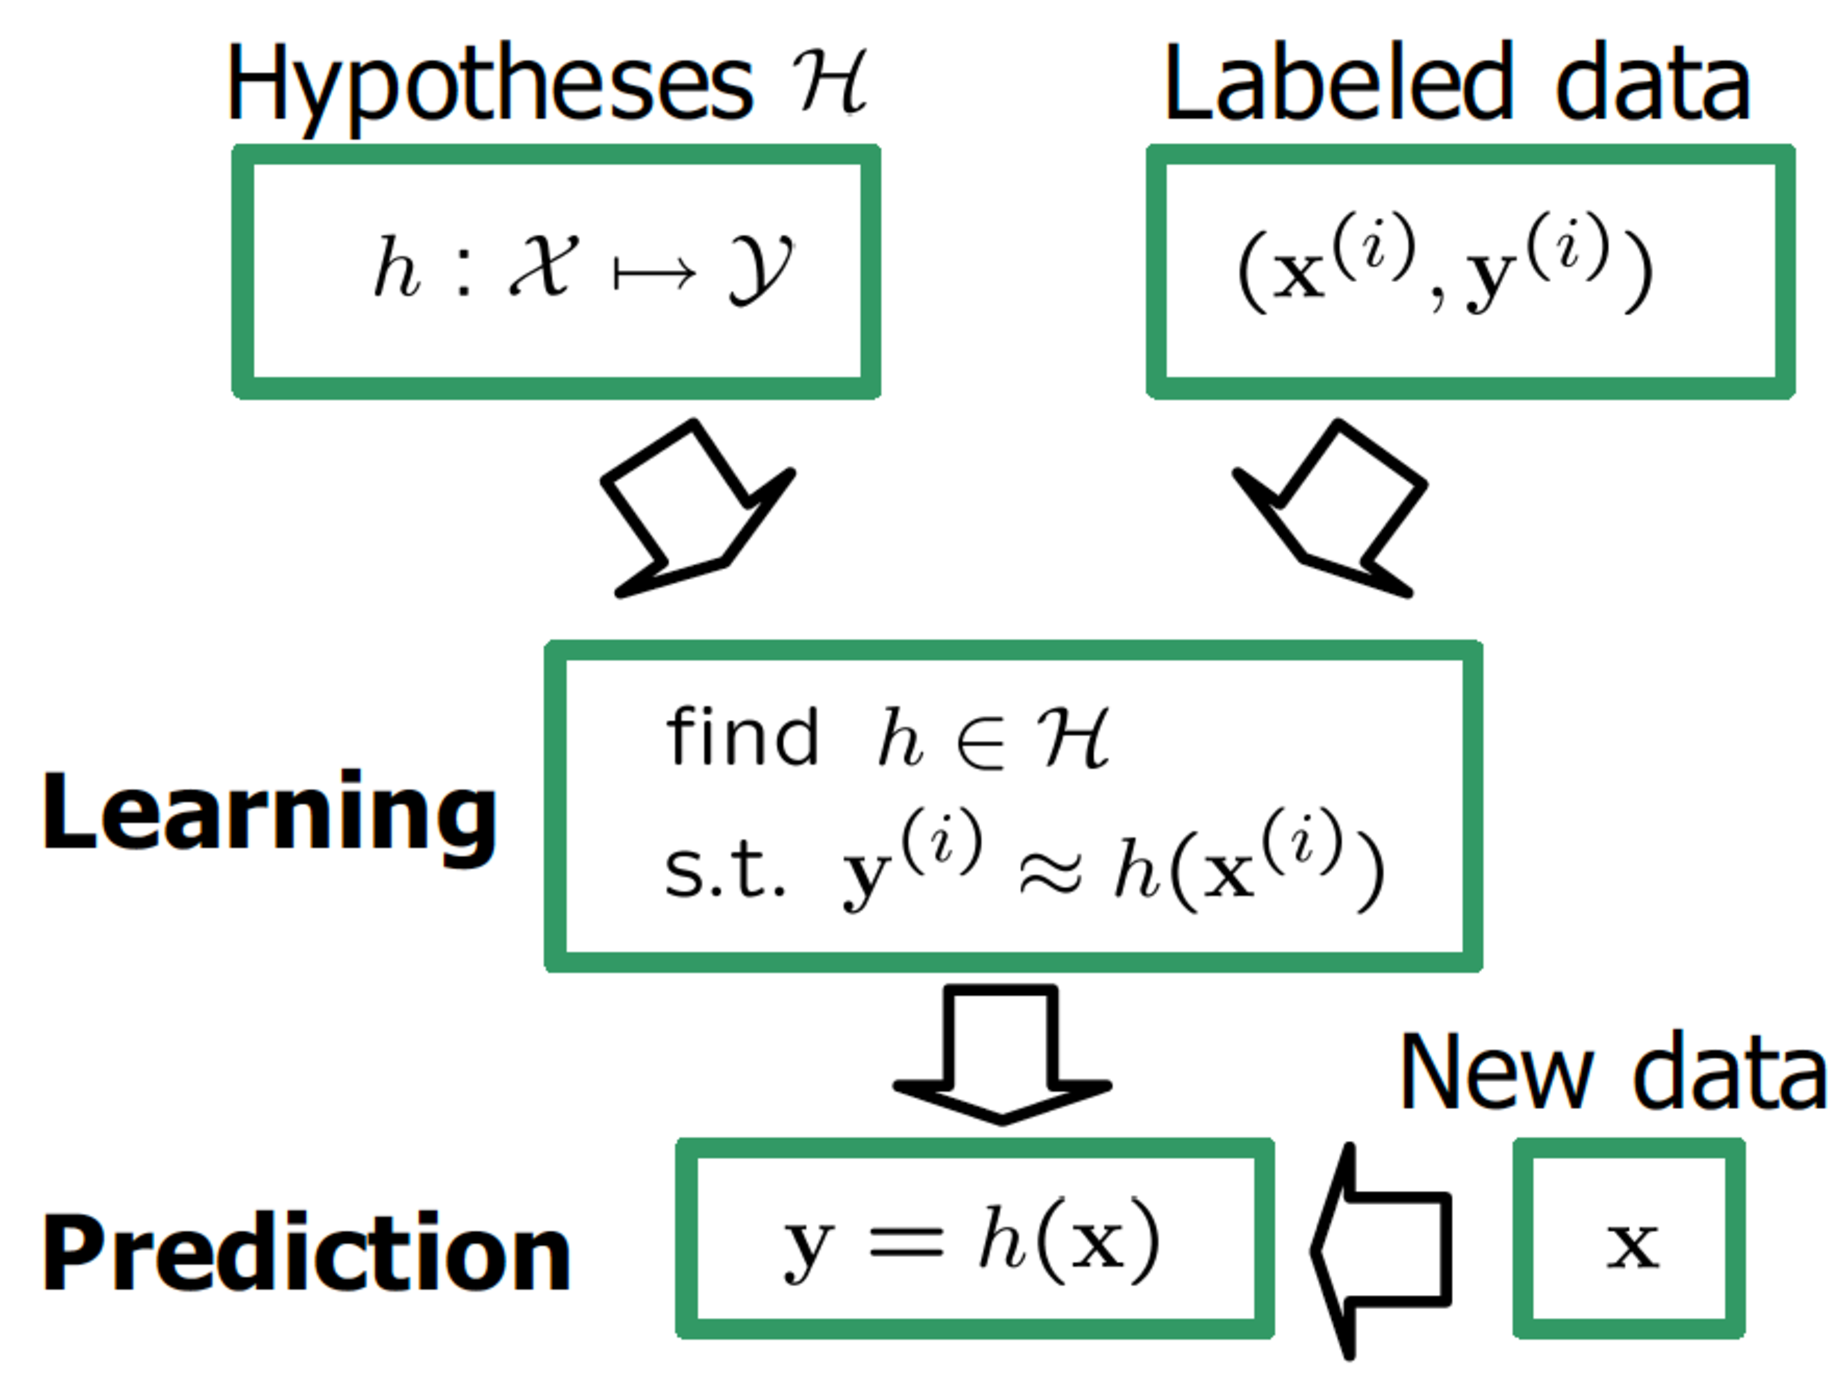
\includegraphics[width=0.80\textwidth]{supervised-learning-hypothesis.pdf}
%\caption{\label{fig:intro-hypothesis}Hypothesis, Generatioalization in
%  Supervised Learning Setting\todo{Current fig is directly copied from
%    Ben Taskar's thesis, redraw it}}
%\end{figure}

In this thesis, following the definition of \kw{bias}
in~\cite{mitchell1980need}, we define \kw{indutive bias} as:

\begin{quote}
  \label{def:bias}
  `Any bias for choosing one generalization over another, other than
  strict consistency with the observed training instances'.
\end{quote}

\subsection{Beyond Training Data: The Origins of Inductive Biases}
\label{ssec:intro:bias-source}
Inductive biases are widely studied in the history of machine
learning. As the definition stated above, inductive biases can be any
assumption beyond the observed training data. In this thesis, we
focused on the supervised learning setting, where observed training
data only means the annotated training data directly avaible to that
task.


For the popular supervised learning setting, let $\mathcal{H}$ refer
to machine learning model families, including deep learning
models. The task of finding a target hypothesis $h$ is reduced to
estimating the model parameters by fitting the training data. Hence,
preferences beyond training data can naturally organized into two
goals: how to choose the hypothesis class $\mathcal{H}$ and how to
find the $h$ is necessary to generalize to new data. For example,
different \kw{model families} can represent different hypothesis
classes. For example, generalized linear models such as logistic
regression and support vector machines, can only support linear
decision boundaries.  Secondly, inductive biases are also used in
\kw{feature engineering}. For data that are not linear seperable, the
choices of \kw{kernel designing} also introduce inductive bias in
kernel-based SVM models. For finding the specific hypothesis $h$,
there are also many assumptions about optimization. For example,
smoothness assumptions in the \kw{optimization} method, such as
Stochostic gradient decent, which was shown to have better
generalization.  \kw{Inference Algorithms}, such as combinatorial
optimization approaches, such as graph cuts, partitions, bipartie
mactching, and dynamic programming can also be involved during the
hypothesis learning, which will also constrain the learning. In this
dissertation, we mainly focus on representation learning. For
inference, we use methods, such as greedy search, maximum spanning
connected graph, and dynamic programming for CKY parsing. Finally, the
biases in the \kw{Training Data} will also influence the hypothesis
finding. It is often the case that available datasets do not exactly
represent the data distribution of interest.  One particularly
problematic case is when the dataset is biased in some way against a
particular demographic group, which often leads to model predictions
that unfairly disadvantage members of that group. Hence, \kw{Data
  manipulation} can also help finding the desired hypoethsis by
augmenting the original training data with inductive biases.

According to the universal approximation
theorem~\citep{hornik1989multilayer}, properly parameterized neural
network can represent any function. Further more, training data seems
rich enough in many cases. It seems purely data-driven deep learning
can learn any target function. Then, what kind of inductive biases we
need in deep learning era? In the following, by two examples of
inductive biases used in computer vision and natural language
processing, we show what are the inductive biases used beyond the
training data in the deep learning era.

\begin{figure}[!th]
  \centering
  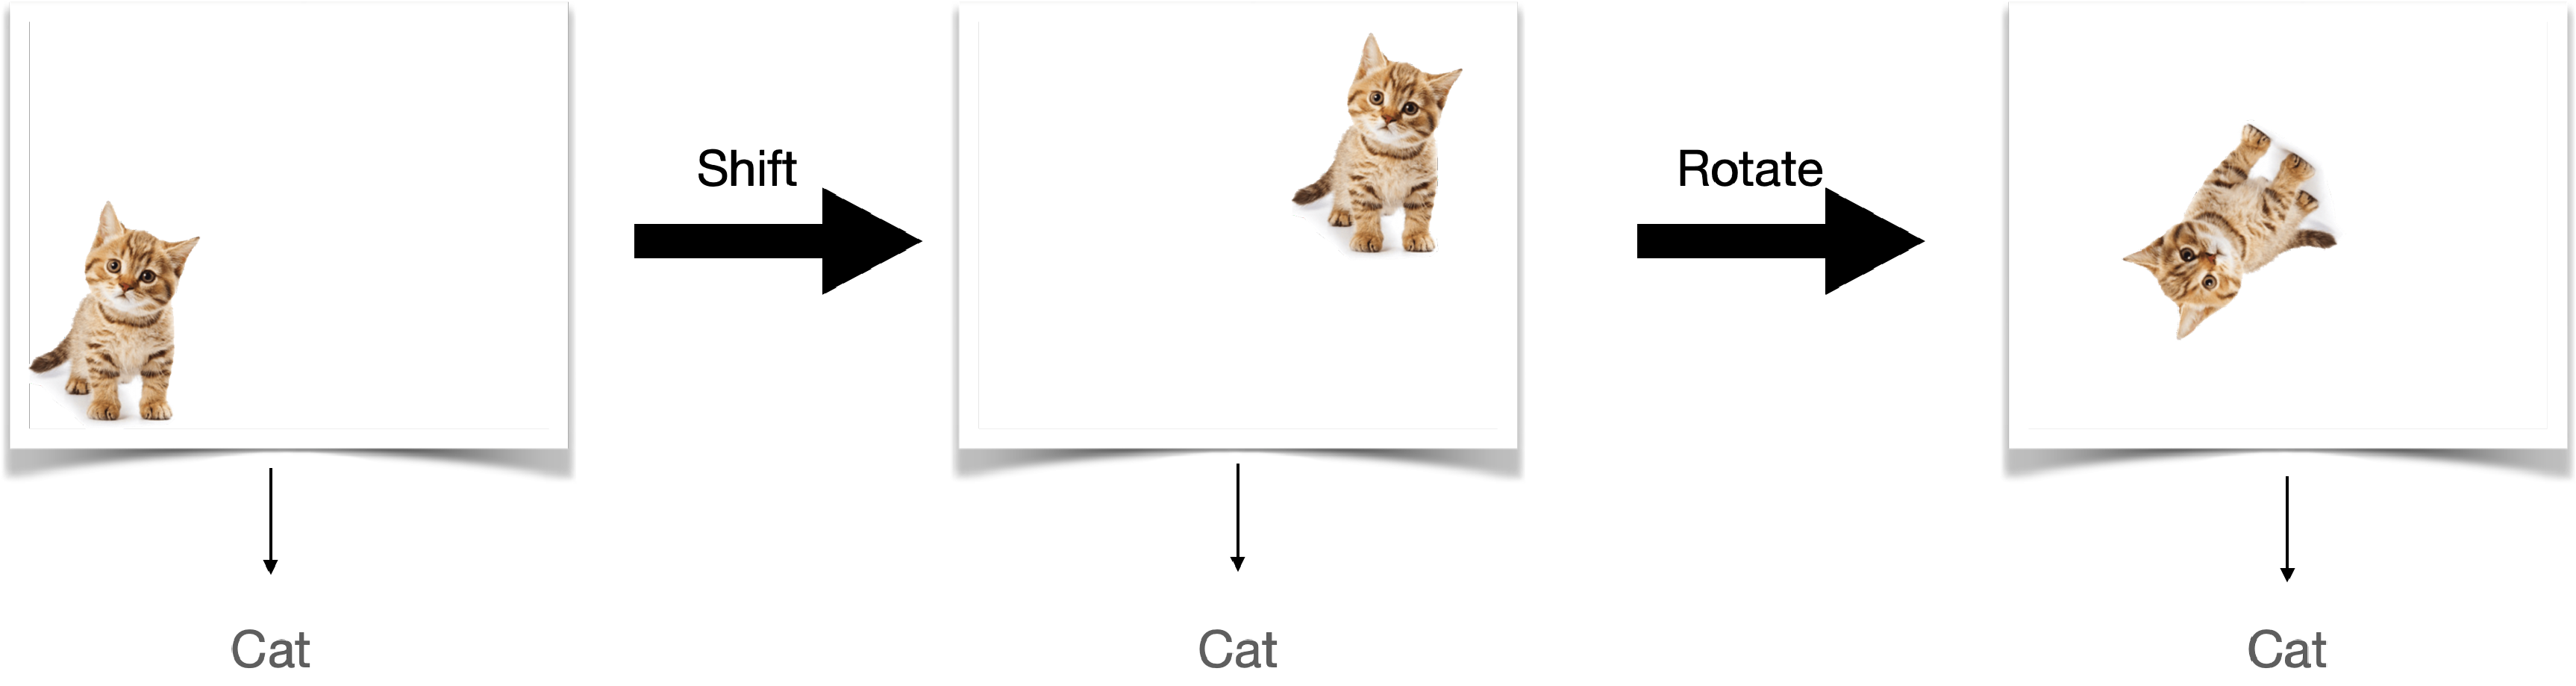
\includegraphics[width=0.98\textwidth]{shift-cat-example.pdf}
  \caption{\label{fig:shift-cat-example}In object classication task,
    we hope the learned model can still recognize `cat' for the unseen
    image with shifted or rotated cat.}
\end{figure}

\begin{figure}[!th]
  \centering
  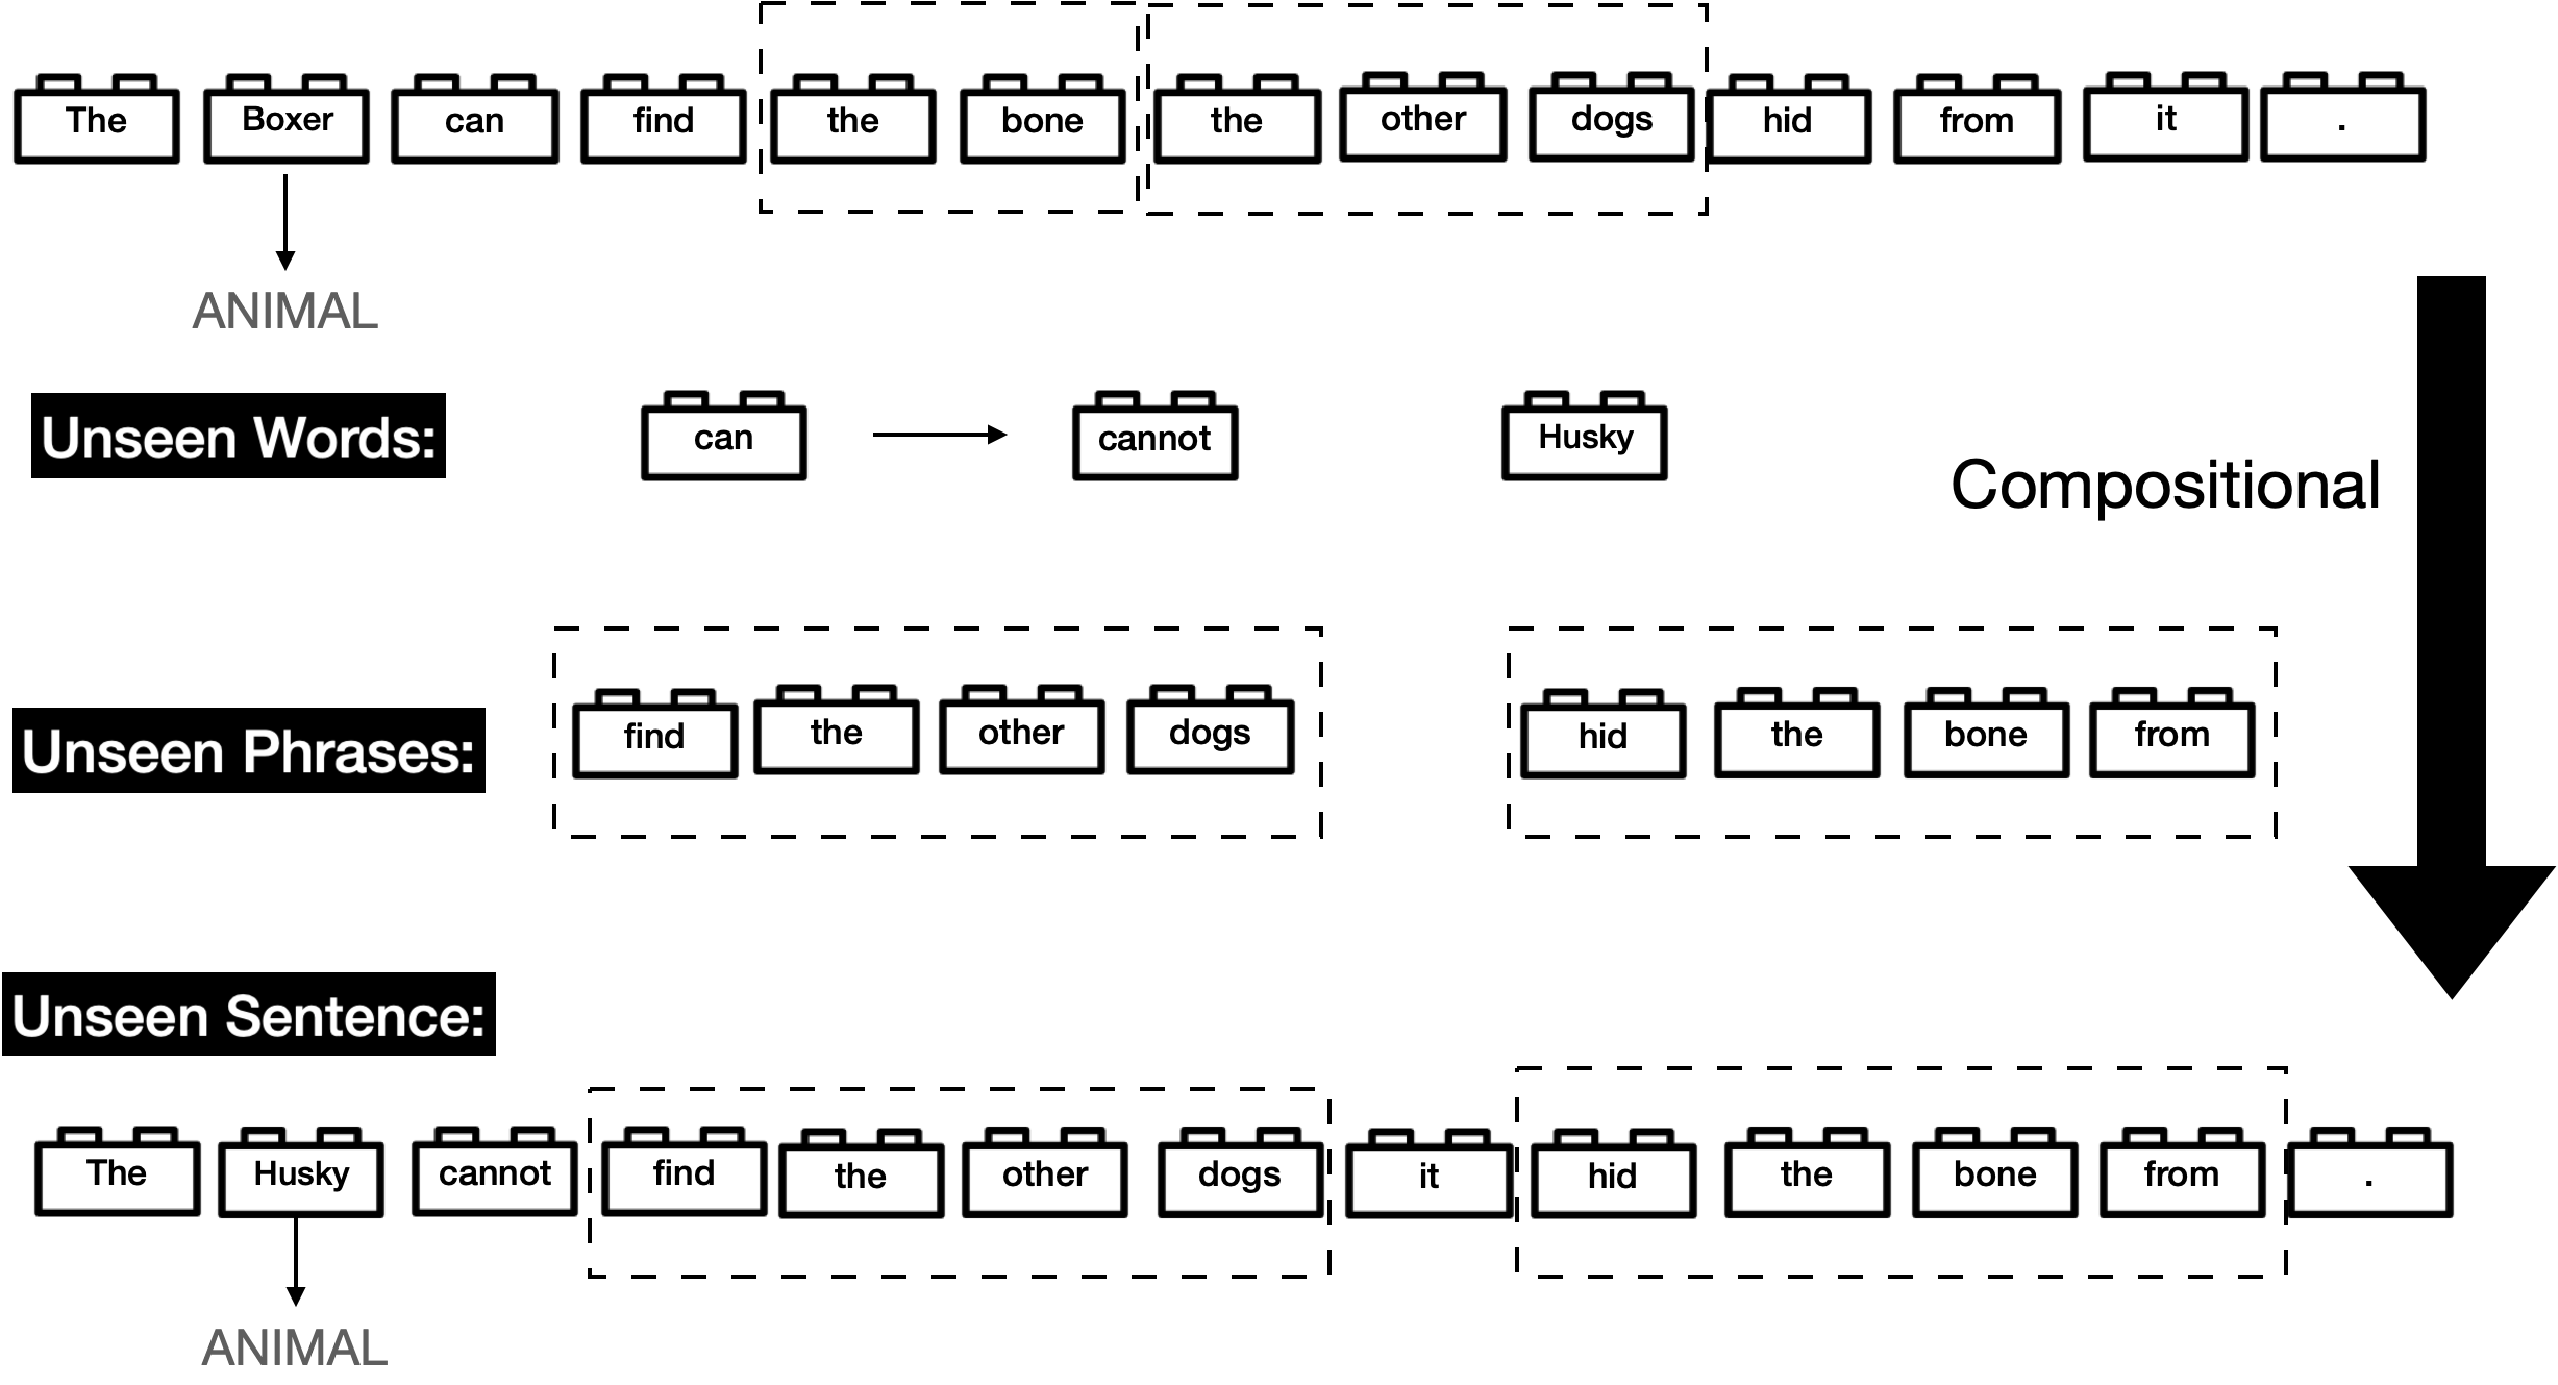
\includegraphics[width=0.98\textwidth]{compositional-dog-example.pdf}
  \caption{\label{fig:compositional-dog-example}In named entity
    recognization task, we hope the learned model can still recognize
    `dog' for new word 'Husky' in unseen context with newly composed
    words, phases and sentences.}
\end{figure}

For example, the
translation invariance for convolutional neural networks~(CNN) and
pooling, and the recurrent assumption of recurrent neural
networks~(RNN), the equivariance over permutation for neural graph
networks~(GNN), the positional encoding for word orders in
Transformer, they are all specific inductive biases.

%\todo{SGD generalization,smoothness}
%\todo{Optimization will control the bias shift during learning}


%For example, naturally occurring data will often
%  underrepresent minority groups, so systems can do well on average
%  while having high error rates on these groups
%
% Datasets may also recapitulate stereotypes tied to historical
%%  injustices, which incentivizes models to learn these very
%  stereotypes to achieve the best test accuracy (Zhao et al., 2017,
%  2018; Rudinger et al., 2018). Training data collected from current
%  users of a system will likely be skewed towards users for which the
%  system works well, leading to a feedback loop in which underserved
%  users become increasingly underrepresented in the training data
%  (Hashimoto et al., 2018).
%\todo{Data augmentation for different pertubation}
%\todo{Realistic distribution shift}
In this thesis, we mainly study inductive biases from neural
architectures and the corresponding representation learning.

\subsection{Inductive Biases for Deep Lingusitic Structured
  Prediction}
\label{ssec:intro:bias-dsp}

For systematic generalization, the search for appropriate inductive
biases is necessary for deep linguistic structured prediction.

Let us denote an observation $x \in \mathcal{X}$. It can be any natural
language text. Such as, the sentence ``The dog cannot find the bone it
hid from the other dogs" or a dialogue segment as shown
in~\autoref{fig:intro-dialogue}. We define an output structured
prediction for $x$ by $y \in \mathcal{Y}(x)$. Here $y$ is a structured
symbolic representation for $x$. For exameple, $y$ could be a sequence
of part-of-speech tags in~\autoref{fig:intro-dog-pos}, a constituent
tree in~\autoref{fig:intro-dog-tree} or a dependency tree
in~\autoref{fig:intro-dog-dep}. It can also be a broad-coverage
meaning representation, like AMR, UCCA, or a dialogue state table. To
represent the target function $y=f(x)$, we adopt the popular
energy-minimization strategy by defining $f(x)$ as the minimizer of an
auxiliary energy optimization problem.
\begin{equation}
\label{eq:argmin}
f(x) = \argmin_{y \in \mathcal{Y}(x)} E(x, y),
\end{equation}
where $E(x,y)$ is a scoring function to represent the energy between
$x$ and a candidate output structure $y$.

In many NLP applications, the candidate output set $\mathcal{Y}(x)$ is
finite but exponentially large, and its size may depend on the input
$x$. For both exact and approximate optimization in
Equation~\ref{eq:argmin}, the main challenges lie on how to model the
representation of \IN~and~\OUT, and the interactions between
them. Practitioners typically employ energy functions with specific
factorization structures to design efficient algorithms, by assuming
the whole energy $E(x, y)$ can be decomposed as a sum of
\textbf{factors} $c$, denoted by $E(x, y) =\sum_{c \in C} E(x, y_{c})$.

A popular choice to represent the factorization is to index both $x$
and $y$ as a set of sub-components $x=(x_{1},..., x_{i},.... x_{N})$
and $y=(y_{1},...y_{j},...y_{M})$. In AMR parsing as shown in
Figure~\ref{fig:intro-dog-amr}, $x_{i}$ can be a word or multi-word
expression in a sentence, while $y_{j}$ can be a single AMR node and
relation.  For dialog state tracking in
Figure~\ref{fig:intro-dialogue}, $x_{i}$ is an utterance in the
dialog, while $y_{i}$ is the value for each intent and slot in the
predicted frames. A factor $c$ may depends on multiple subcomponents
of $x$ and $y$.

The interdependence assumptions between those sub-components in $x$
and $y$ are key in structured prediction model. In the
\autoref{chap:background}, we show various representation formalism
~(such as graphical models), structured learning~(max-margin
framework) and inference approaches~(dynamic programming, integer
linear programming) to model the interdependence. Inductive biases can
be designed in all the three key aspects.

In this thesis, we always assume the \kw{indenpendence factorization}
paradigm, where each factor $c$ only depends on a well-segemented
subset of subcomponents $y_{c}$ and the aligned $x$
components~(anchors)~$x_{c}=a(y_{c})$. In other words, the output
parts, once decomposed into mutually exclusive output segments, we
consider each segment as an atomic output part, and each atomic part
are independent from each other.

\begin{equation}
    \label{eq:independent-factor}
    \begin{split}
    E(x, y) & =\sum_{c \in C} E(x, y_{c}) = \sum_{c \in C}E(x, a(y_{c}), y_{c})  \\
    \end{split}
\end{equation}

Here, $a(y_{c})$ is the alignment model to find how independent output
parts $y_{c}$ are \kw{anchored} to the constituents of the observation
$x$. Thus the prediction of each $y_{c}$ are independent from each
other, and can be locally decided by its aligned anchors.

Hence, this simple independent factorization can decompose the
structured learning into decomposed local learning~(constrained by
some global constraints). More importantly, it also makes the
inference tractable, thus can be easily employed in the end-to-end
neural network training framework.

Using AMR parsing in \autoref{fig:intro-dog-amr} as an example, the
independent factorization will first segment the output $y$ into small
parts $y_{c} \in seg_{out}(y)$, then find the anchors $x_{c}$ in the
input sentence for each $y_{c}$ from the candidate decomposition set
$seg_{in}(x)$. For example, one of the segmented $y_{c}$ in
Figure~\ref{fig:intro-dog-amr} is a pre-categorized sub-graph
`(possible-01 :polarity -)', and its anchor $a(y_{c})$ is the anchor
word `cannot'. The words `the', 'from' are mapped to empty nodes.

\begin{figure}[!th]
\centering
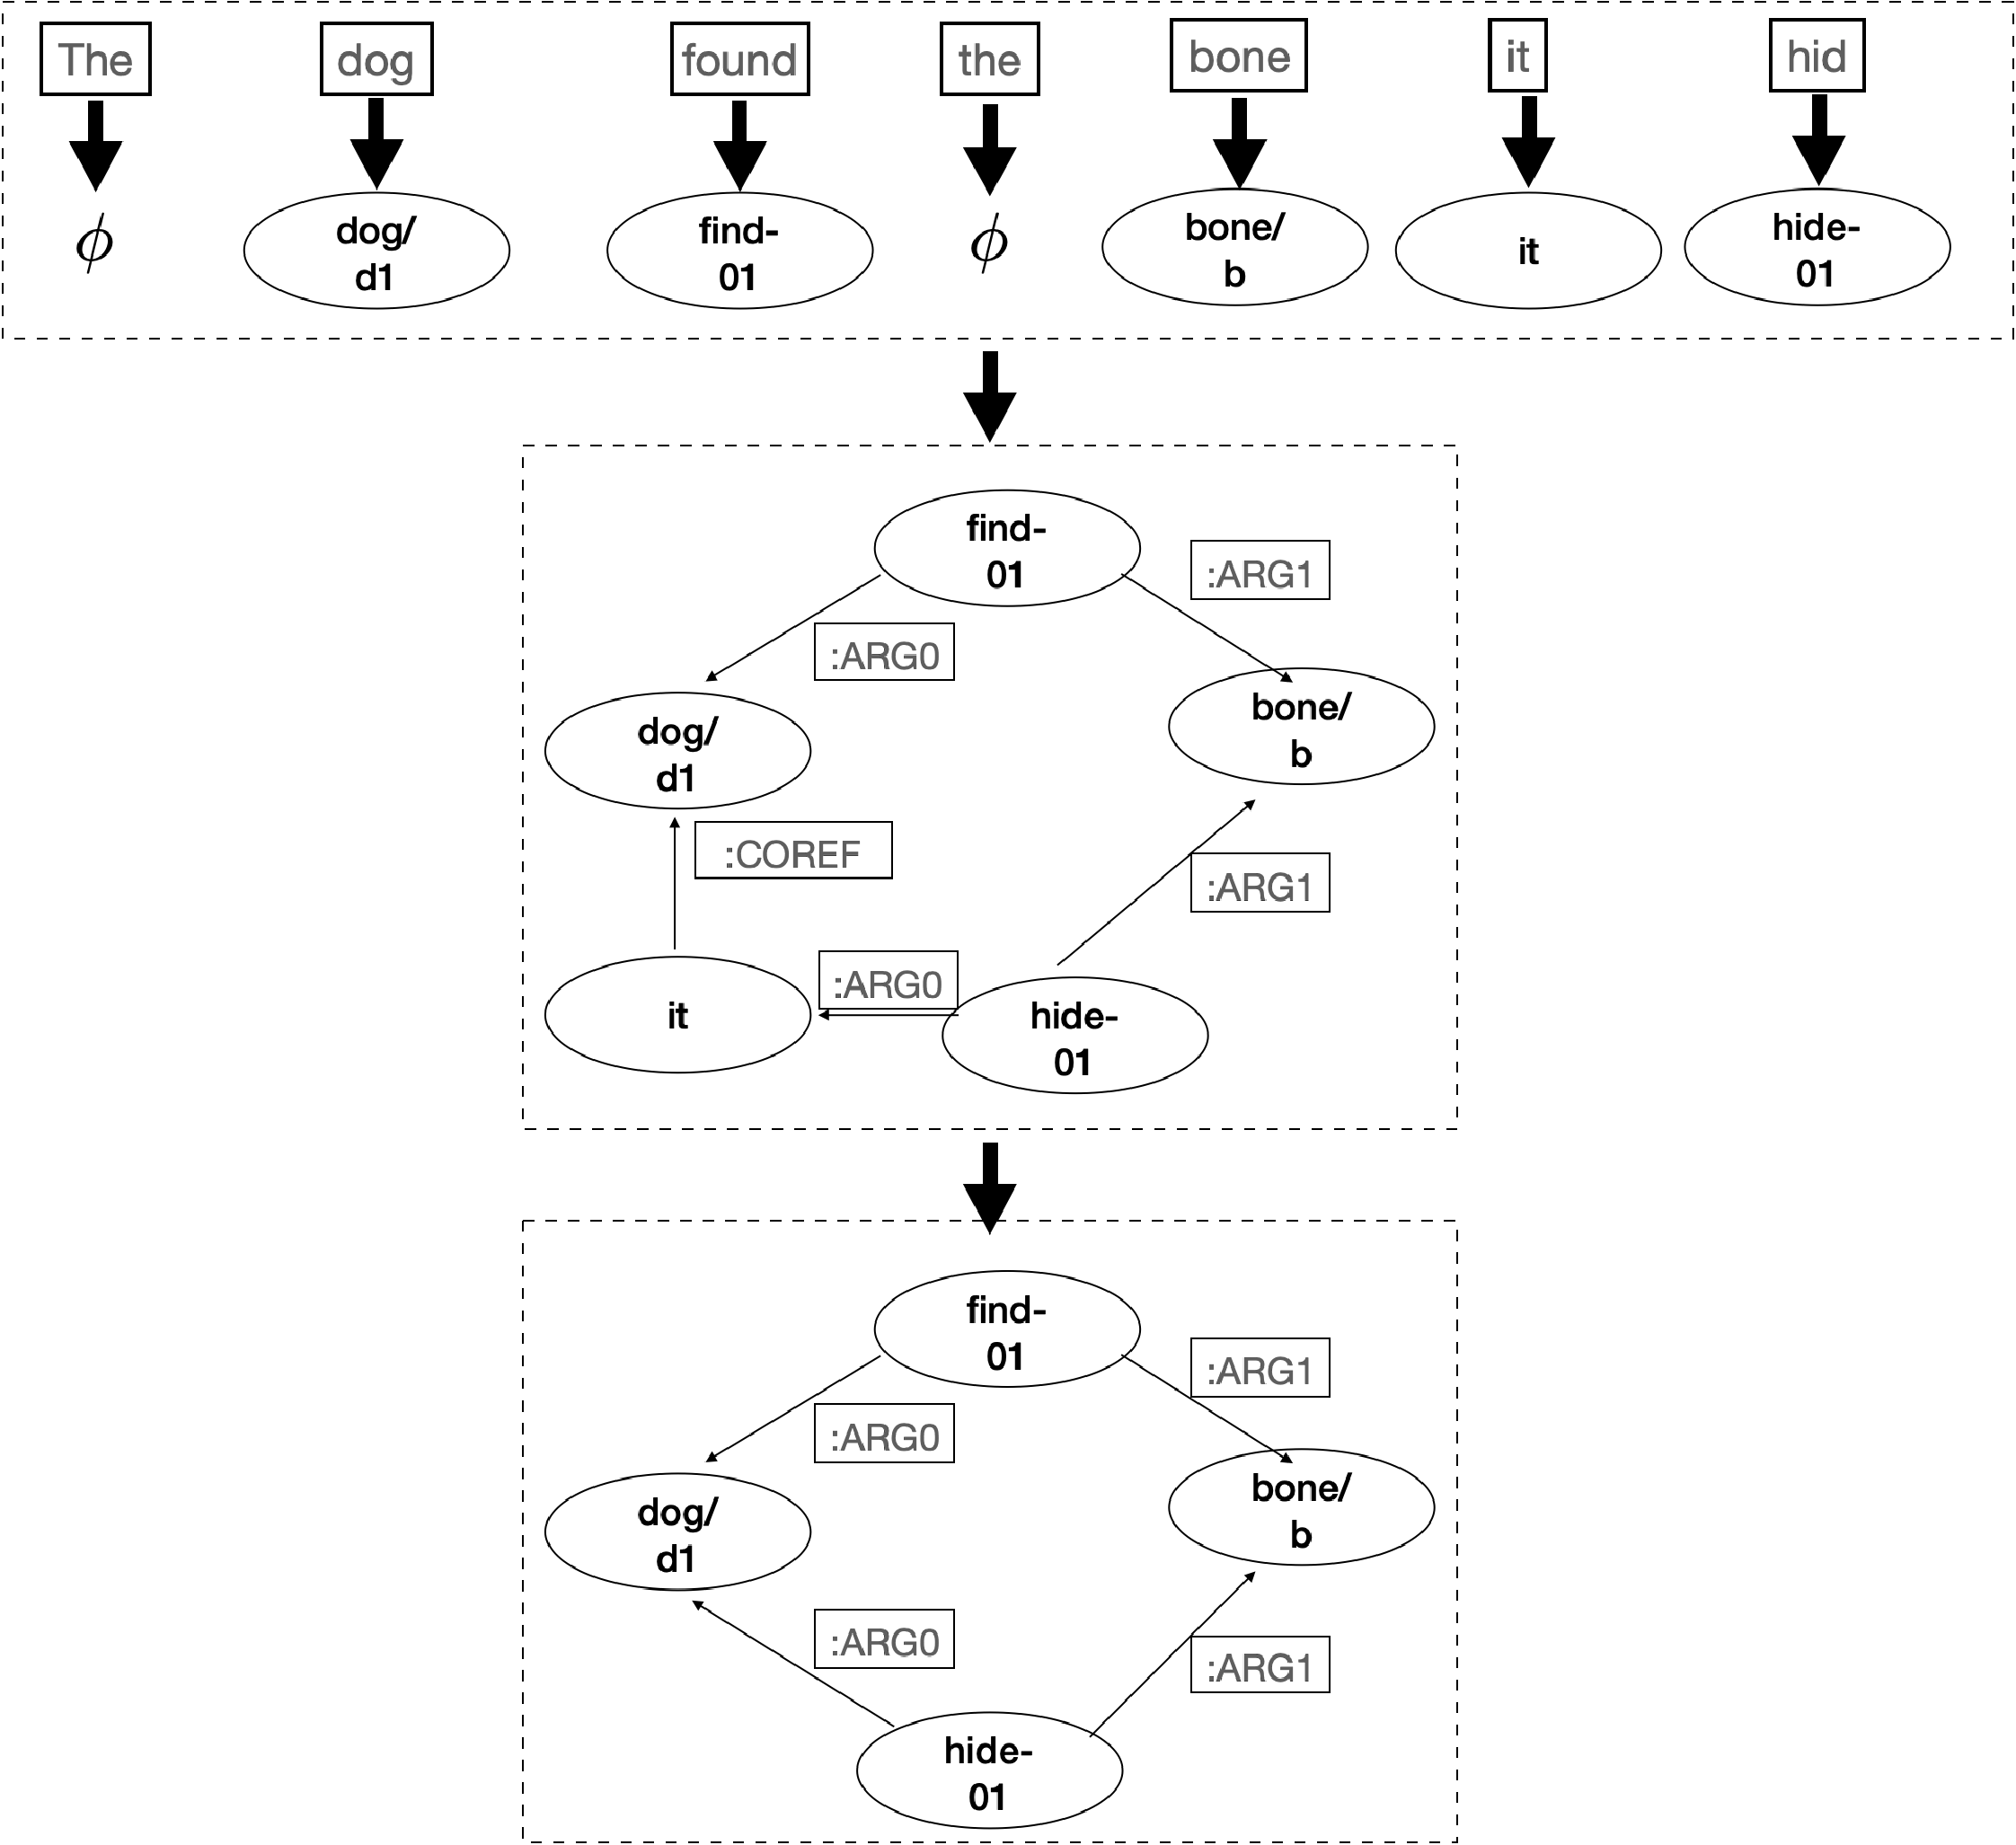
\includegraphics[width=0.80\textwidth]{dog-independent-example.pdf}
\caption{\label{fig:intro-independent-example}Independence
  Factorization for parsing a new sentence "The dog found the bone it
  hid" into an AMR graph}
\end{figure}

During inference, we can directly produce $y_{c}$ for all candidates
segments in a new sentence as shown in
Figure~\ref{fig:intro-independent-example}. We first prepare a list of
candidate anchors $seg_{in}(x)=\{${`The', `dog', `found', `the',
  `bone', `it', `hide'$\}$, then the model will produce the
  independent prediction $y_{c}$ of each anchor as
  $\{\phi,\text{`dog'}, \text{`find-01'}, \phi, \text{`bone'},\text{`it'},
  `hide'\}$, then we assemble the non-empty $y_{c}$ by predicing the
  relations between each other and finally forms \OUT~via
  postprocessing\footnote{The post-processing include mergeing
    coreference nodes~(as the `dog' and `it'), adding other
    attributes}.

  Hence, in the independence factorization setting, the problem is
  reduced into three challenges:
\begin{itemize}
\item How to decompose the output $y$ into a set of independent parts
  $y_{c}$.

\item How to decompose $x$ and derive the aligned input $x_{a_{y_{c}}}$ at the index $a_{y_{c}}$.

\item How to model the representation of $x$ at the index $a_{y_{c}}$ and $y_{c}$ to
  compute the energy score $E(x, a(y_{c}), y_{c})$.
\end{itemize}

The first question on independently decomposing $y$ is either
straightforward or has been resolved by previously existing methods in
our studied tasks. We mainly focus on the remaining challenges on
modeling alignment and representation learning.

%%% Local Variables:
%%% mode: latex
%%% TeX-master: "../../thesis-main.ltx"
%%% End:
